\section{Robustness of the methodology}
\label{sec:robustness}

%\begin{summary}
%In this chapter, we will show that the proposed methodology with the associated algorithms are robust. We will use classical indicator of the field to show that convergence and diversity properties are respected despite the complexity of designing 3D-SIC and the heterogeneous nature of the criteria.
%\end{summary}

%Associated publications:
%\begin{itemize}
%\item N.A.V. Doan, D. Milojevic, F. Robert, Y. De Smet, "A MOO-based methodology for designing 3D-stacked integrated circuits", \textit{Journal of Multi-Criteria Decision Analysis}, vol.21, no. 1-2, pp. 43-63, January-April 2014
%\end{itemize}

%\section{Introduction}
%In the previous section, we have shown how a 3D-SIC can be modelled as an optimization problem and we have applied a NSGA-II metaheuristic. The obtained results indicate that multi-objective optimization can give qualitative and quantitative information to a designer that would not be available with current design tools.

In this section we will take a deeper look at the results of the multi-objective optimization steps. We will analyse the properties of the design space in order to have the view over the convergence and the robustness of our methodology the classical performance indicators used in the field (see Chapter \ref{cha:rol.mcda}).

The following results have been obtained with 5 independent runs. The set of non-dominated solutions over all the simulations will constitute the reference set $R$ for the \textit{epsilon} and the hypervolume indicators. Also, these results have been simulated with all the five criteria presented in Section \ref{sec:crit} instead of only the three first for the case study of Section \ref{sec:casestudy}.

% Other convergence-based indicators such as the generational distance, the $\epsilon$-indicator, a cardinality measure and a distance measure cannot currently be applied for our problem since we do not have a reference set to compare to.

\subsection{Contribution indicator}

The Table \ref{tab:contrib} and the Figure \ref{fig:contrib} show the evolution of the averaged contribution indicator over the iterations for the 5 runs. We see that for the first iterations, $Cont(PO_i/PO_{i-1})$ is greater than 0.5, which means that the algorithm does indeed improve the solutions, then for the last iterations, the indicators are lower than 0.5 which means that there is a convergence.

\begin{table}[h!]
\begin{center}
\begin{tabular}{|c|c|}
\hline Iteration & $Cont(PO_i/PO_{i-1})$ \\ 
\hline 1 & 0.7626 \\ 
\hline 2 & 0.8510 \\ 
\hline 3 & 0.8917 \\ 
\hline 4 & 0.8788 \\ 
\hline 5 & 0.8295 \\ 
\hline \dots & \dots \\
\hline 38 & 0.4522 \\
\hline 39 & 0.3870 \\ 
\hline 40 & 0.2369 \\
%\hline 1 & 0.8080 \\ 
%\hline 2 & 0.8549 \\ 
%\hline 3 & 0.8916 \\ 
%\hline 4 & 0.8734 \\ 
%\hline 5 & 0.8451 \\ 
%\hline \dots & \dots \\
%\hline 38 & 0.4566 \\
%\hline 39 & 0.2741 \\ 
%\hline 40 & 0.3692 \\
\hline 
\end{tabular} 
\end{center}
\caption{Evolution of the contribution indicator}
\label{tab:contrib}
\end{table}

\begin{figure}[h!]
\begin{center}
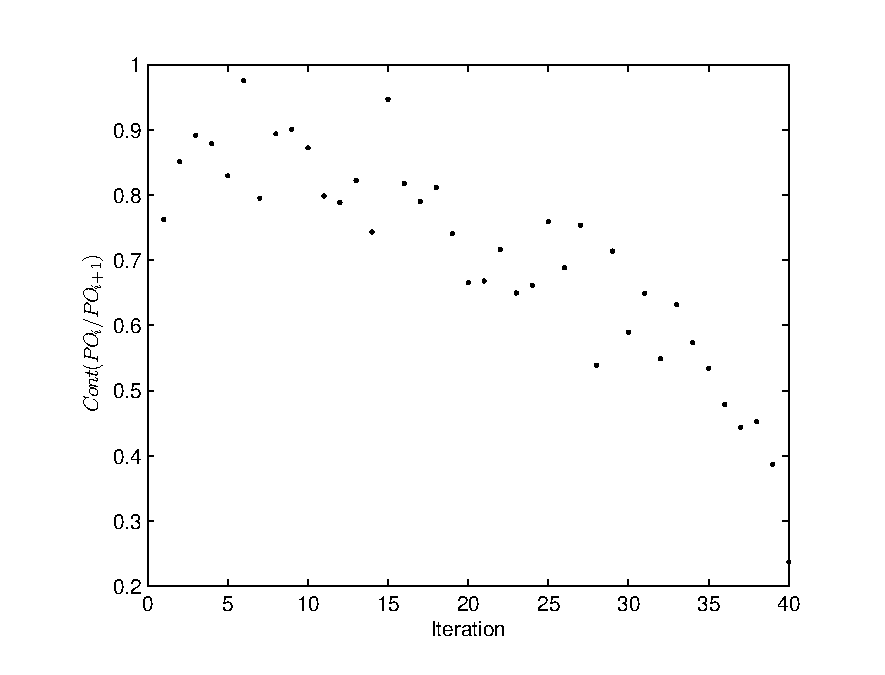
\includegraphics[width=1\linewidth]{contrib2new.eps}
\end{center}
\vspace{-0.5cm}
\caption{Evolution of the contribution indicator}
\label{fig:contrib}
\end{figure}

\subsection{Spread indicator}
\label{app:spread}

The Figure \ref{fig:spread_indicator} shows the results of the spread indicator $I_s$ function of the neighbourhood indicator $\sigma$ (all the 5 runs share the same graph shape). We see that the Pareto front is well spread: if  we consider $I_s \geq 0.9$ we have $\sigma < 0.35$ in average for the 5 runs (normalized values), so we can consider that the algorithm produces a well-spread approximation of the Pareto front.
%Knowing that the extreme (Euclidean) distance between two solutions is equal to 332 (for normalized values), we can consider that the algorithm produces a well-spread approximation of the Pareto front.

\begin{figure}[h!]
\begin{center}
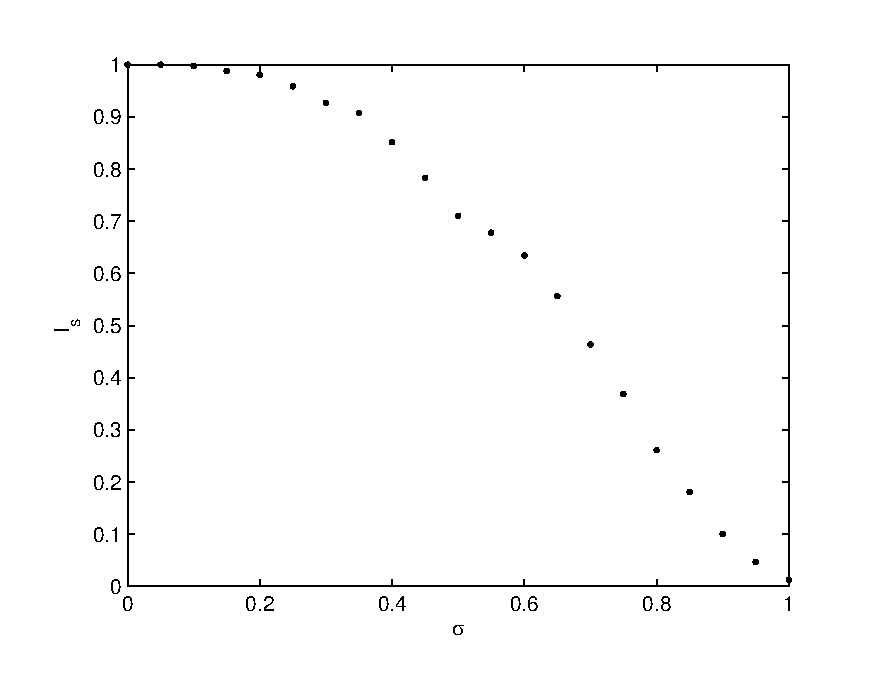
\includegraphics[width=1\linewidth]{spread_indicator_norm2.eps}
\end{center}
\vspace{-0.5cm}
\caption{Spread indicator $I_s$ function of the neighbourhood parameter $\sigma$}
\label{fig:spread_indicator}
\end{figure}

\subsection{Binary $\epsilon$-indicator}
The non-dominated set computed from all the runs will constitute the reference set $R$ that will serve to show the evolution of the $\epsilon$-indicator over time. This evolution is shown in Table \ref{tab:biepsref} (for averaged values after each 10 iterations). We can see that in the first iterations, $I_\epsilon(A,R) > 1$ and $I_\epsilon(R,A) \approx 1$ which means that the front is improved while in the last iterations, $I_\epsilon(A,R) > 1$ and $I_\epsilon(R,A) > 1$ which shows convergence.

A comparison of the binary $\epsilon$-indicators between each experiment (after convergence) is also given, in Table \ref{tab:biepsxp}. We can see that $I_\epsilon(A,B) > 1$ and $I_\epsilon(B,A) > 1$ which indicates that neither $A$ weakly dominates $B$ nor $B$ weakly dominates $S$. This means that the generated front is consistent from one experiment to another.

Also, in Table \ref{tab:biepsiter} are given the $\epsilon$-indicator between iterations of an experiment (the same observations apply for the other runs). We can see that in the first iterations, the front is always improved ($I_\epsilon(A_i, A_{i-1}) > 1$ and $I_\epsilon(A_{i-1}, A_i) \leq 1$) while in the last iterations, it begins to converge ($I_\epsilon(A_i, A_{i-1}) > 1$ and $I_\epsilon(A_{i-1}, A_i) > 1$).

\begin{table}[h!]
\begin{center}
\begin{small}
\begin{tabular}{|c|c|c|}
\hline Iteration & Averaged $I_\epsilon(A,R)$ & Averaged $I_\epsilon(R,A)$\\
\hline 1 & 5.5255 & 1.0178\\
\hline 10 & 4.4307 & 1.0235\\
\hline 20 & 3.8102 & 1.1023\\
\hline 30 & 2.3614 & 1.1234\\
\hline 40 & 1.6569 & 1.2381\\
\hline
\end{tabular}
\end{small}
\end{center}
\caption{Evolution of the binary $\epsilon$-indicator (averaged values compared to the reference set $R$) over time}
\label{tab:biepsref}
\end{table}

\begin{table}[h!]
\begin{center}
\begin{footnotesize}
\begin{tabular}{|c|c|c|c|c|c|}
\hline $I_\epsilon(A,B)$ & Run 1 & Run 2 & Run 3 & Run 4 & Run 5 \\ 
\hline Run 1 & 1 & 1.7270 & 1.3594 & 1.8664 & 1.2542 \\ 
\hline Run 2 & 1.5713 & 1 & 1.4122 & 1.7791 & 1.3420 \\ 
\hline Run 3 & 1.4737 & 1.8638 & 1 & 1.9268 & 1.3069 \\ 
\hline Run 4 & 1.3436 & 1.4564 & 1.2843 & 1 & 1.2365 \\ 
\hline Run 5 & 1.4214 & 1.7650 & 1.3918 & 1.7545 & 1 \\ 
%\hline Run 1 & 1 & 1.7234 & 1.3772 & 1.8880 & 1.2152 \\ 
%\hline Run 2 & 1.5305 & 1 & 1.3548 & 1.8333 & 1.3488 \\ 
%\hline Run 3 & 1.4409 & 1.9285 & 1 & 1.8305 & 1.2952 \\ 
%\hline Run 4 & 1.3709 & 1.4048 & 1.2654 & 1 & 1.2310 \\ 
%\hline Run 5 & 1.4554 & 1.8533 & 1.4400 & 1.7868 & 1 \\ 
\hline 
\end{tabular} 
\end{footnotesize}
\end{center}
\caption{Comparison of the binary $\epsilon$-indicators for each experiment}
\label{tab:biepsxp}
\end{table}

\begin{table}[h!]
\begin{center}
\begin{tabular}{|c|c|c|}
\hline Iteration & $I_\epsilon(A_i, A_{i-1})$ & $I_\epsilon(A_{i-1}, A_i)$ \\ 
\hline 1 & 1.6674 & 1.1053 \\ 
\hline 2 & 1.7223 & 1 \\ 
\hline 3 & 2.4439 & 1 \\ 
\hline 4 & 1.7477 & 1 \\ 
\hline 5 & 2.0577 & 1 \\ 
\hline \dots & \dots & \dots \\
\hline 38 & 1.8788 & 1.4916 \\
\hline 39 & 1.5344 & 1.8065 \\ 
\hline 40 & 1.9862 & 1.6609 \\
\hline 
\end{tabular} 
\end{center}
\caption{Comparison of the binary $\epsilon$-indicators between iterations of the same experiment}
\label{tab:biepsiter}
\end{table}

\subsection{Unary hypervolume indicator}
The evolution of the hypervolume (averaged values) is given in Table \ref{tab:hypervolref} and in Figure \ref{fig:hypervolref}. We can see that the value is (linearly) increasing over time, reaching convergence in the last iterations where the value stabilizes.

The result for each experiment is also given, in Table \ref{tab:hypervol} and the used reference point is the worst point computed from all the sets for normalized data. As we can see, the values are rather consistent from one run to another.

\begin{table}[h!]
\begin{center}
\begin{tabular}{|c|c|}
\hline Iteration & Averaged hypervolume \\
\hline 1 & 0.0574 \\
\hline 10 & 0.0701 \\
\hline 20 & 0.0876 \\
\hline 30 & 0.0931 \\
\hline 40 & 0.1036 \\
\hline
\end{tabular}
\end{center}
\caption{Evolution of the unary hypervolume indicator (averaged values compared to the reference set $R$) over time}
\label{tab:hypervolref}
\end{table}

\begin{figure}[h!]
\begin{center}
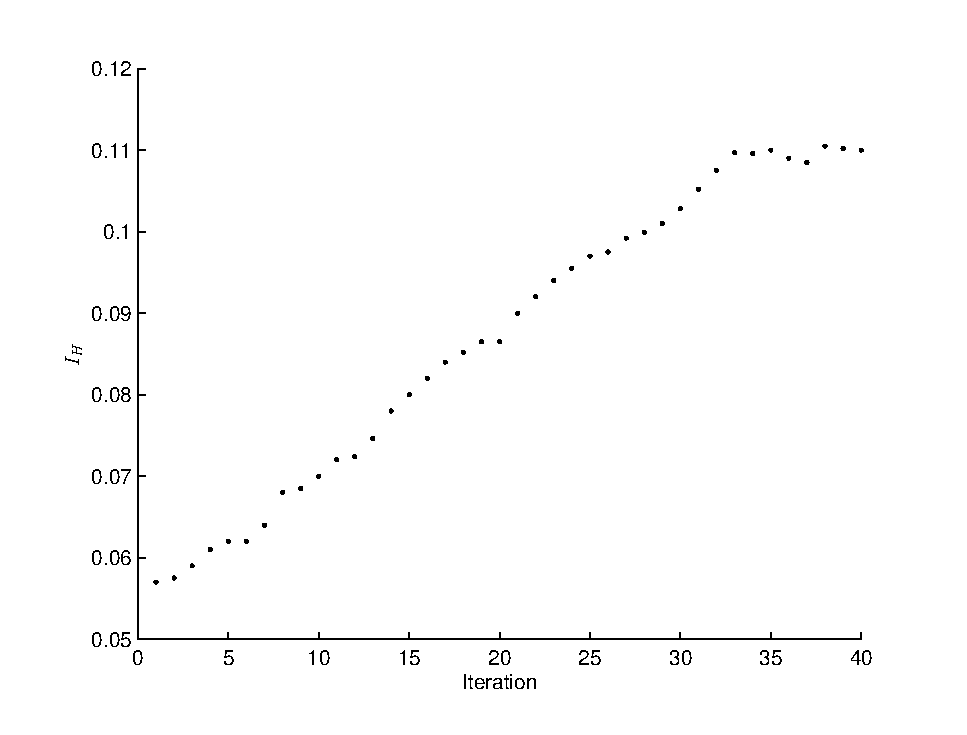
\includegraphics[width=1\linewidth]{hypervolref2.eps}
\end{center}
\vspace{-0.5cm}
\caption{Evolution of the unary hypervolume indicator (averaged values compared to the reference set $R$ over time}
\label{fig:hypervolref}
\end{figure}

\begin{table}[h!]
\begin{center}
\begin{tabular}{|c|c|}
\hline Run & $I_H$\\
\hline 1 & 0.1171\\
\hline 2 & 0.1105\\
\hline 3 & 0.1015\\
\hline 4 & 0.1185\\
\hline 5 & 0.0939\\
%\hline 1 & 0.084617\\
%\hline 2 & 0.084566\\
%\hline 3 & 0.094522\\
%\hline 4 & 0.102438\\
%\hline 5 & 0.101421\\
\hline 
\end{tabular}
\end{center}
\caption{Hypervolume for each experiment}
\label{tab:hypervol}
\end{table}

\subsection{Density of the Pareto front - gaps in the frontier}
Another indicator of the Pareto front structure is its density. Here we will measure the density by finding gaps in the frontier. This will be done by counting the number of solutions in the neighbourhood of another solution. Since the extreme distance between two solutions is 450.364 in average for the 5 runs (non-normalized), we consider that an acceptable neighbourhood is twice the distance between two solutions if all the solutions were equidistant. We have thus a neighbourhood of about 2. This test has shown that there was always at least one solution near another one, even for a neighbourhood of 1, meaning that the algorithm can produce a sufficiently dense frontier.

%\subsubsection*{Binary hypervolume indicator}
%The binary hypervolume indicator $I_{H2}(A,B)$ is defined as the hypervolume of the subspace that is weakly dominated by $A$ but not by $B$. A value closer to 0 means that $B$ is a better approximation \cite{1197687}.

\subsection{Convexity indicator}
%The convexity is also an indicator of the structure. Globally, the Pareto front is not convex, as one may expect since the heterogeneous nature of the criteria. However, the frontier appear to be partially convex and this convexity also depends on the set of criteria that are considered. This is probably due to some correlation between the criteria but this is still to be investigated more deeply since the convexity properties can have an impact on the choice of the multicriteria method to use.
The convexity is also an indicator of the structure, so analyses have been performed to determine the shape of the Pareto front. Globally, the Pareto front is not convex, as one may expect given the heterogeneous nature of the criteria and correlation between them. Also, since an approximate algorithm has been used, small gaps between solutions may exist that will not give a convex shape to the frontier.

%\section{General properties of the algorithm}

\subsection{A word on the scalability of the methodology}
The previous results have been obtained with the case study shown in Section \ref{sec:casestudy}. Similar results can be obtained for the scaled case study of Section \ref{sec:casestudyscale} which contains about a hundred blocks, and it has also been successfully tested for a few hundreds of randomly-generated blocks. Reaching several hundred to a thousand of blocks, the algorithm starts to take tens of minutes per iteration which shows its limits in terms of scalability even though convergence can still be shown.

\section{Conclusion}

In this chapter, we have proposed a 3D-SIC model that can take into account 5 different criteria to apply MOO with a more global multi-criteria analysis. To the best of our knowledge, current tools deal with a limited set of criteria (usually 3) and only perform trade-off analyses. We have performed simulation on two different case studies and the results have shown interesting information that can be relevant for a designer. First, using a multi-objective optimization methodology does not only consider all the criteria at the same time but also proceed to an extensive design space exploration which is rarely done with current tools. Second, the qualitative results shown here can give relevant information to the designer and they can even be quantified with a more accurate model. Third, the flexibility of MOO allows to easily consider new degrees of freedom, such as the form factor of the blocks and the heterogeneity, without having to change the paradigm. Finally, we have validated the methodology with a scaled case study and shown that a multi-objective optimization gives added values compared to a uni-criterion paradigm.

We have then shown that the proposed methodology has proved to be robust even if the problem contains criteria of heterogeneous nature. With the several indicators that we have analysed, we can conclude that the algorithm we used can show good properties of convergence, spread and density.
%For information purposes, we have also computed less state-of-the-art indicators: the contribution indicator and the spread indicator, as defined in \cite{talbi09}. These results are presented in Appendices \ref{app:cont} and \ref{app:spread} and we can see that they also reflects the good convergence and diversity of the algorithm.

In the next chapter, we will show how these results can be exploited, with a multi-criteria point of view, to help a designer make a choice among a set of efficient solutions.

%\section{Conclusion}
%
%In this chapter we have shown that the used methodology has proved to be robust even if the problem contains criteria of heterogeneous nature.

%With these results, we believe that a multi-criteria paradigm can be applied to the design of 3D-SICs in order to produce them more efficiently than what can be done with the current tools.

%Globally, our methodology includes two steps:
%\begin{itemize}
%\item Fast design space exploration and performance estimation/optimization using metaheuristics
%\item Ex-post exploration for multi-criteria decision analysis and decision over the most-suitable solutions
%\end{itemize}
%This work has focused on the first step. As future works, the second step is still to be done. Indeed, now that we can generate a Pareto front, we have to fully analyze how the information provided by the frontier can be used by a designer with an ex-post exploration. As for the criteria, they will be improved continuously in order to be able to have more accurate estimation.

%It is worth to stress that we have done this work for a real case study but it will also be interesting to see how this methodology can be used on other structures, especially when there is a scaling effect on the number of components. Finally, this research will be validated by integration to existing design flow such as PathFinding \cite{DBLP:conf/3dic/MilojevicCCRRSAPM09}. This will allow us to work with a complete flow, from architecture/system-level to physical design and to compare this methodology with the current classical ones.

%These two processes constitute a research field on their own and will need extensive future works. For instance, if many criteria are involved, it can be long and difficult to efficiently establish the Pareto frontier since many of the explored solutions can be efficient solutions, as highlighted in~\cite{Farina02, Stanojevic08}. Also, a graphical decision space might be unusable with many criteria since no relevant information can be visualized, as shown in~\cite{Stanojevic08}. These issues are being studied and one promising way to overcome them is to integrate the preference model in the solution space exploration process~\cite{1569979, Branke04, Cvetkovic00}. In addition, the establishment of a preference model of a designer in relation with several criteria is another research field which also constitute a future work.

%We believe that with these promising results of our first approach, it will be possible to efficiently design 3D-SICs using MCDA tools.
